%%%%%%%%%%%%%%%%%%%%%%%%%%%%%%%%%%%%%%%%%%%%%%%%%%%%%
% settings                                          %
%                                                   %
% einbinden mit: %%%%%%%%%%%%%%%%%%%%%%%%%%%%%%%%%%%%%%%%%%%%%%%%%%%%%
% settings                                          %
%                                                   %
% einbinden mit: %%%%%%%%%%%%%%%%%%%%%%%%%%%%%%%%%%%%%%%%%%%%%%%%%%%%%
% settings                                          %
%                                                   %
% einbinden mit: \input{settings}                   %
%%%%%%%%%%%%%%%%%%%%%%%%%%%%%%%%%%%%%%%%%%%%%%%%%%%%%

\documentclass[a4paper, 11pt, oneside, openany,abstracton]{scrreprt} % koma-script layout

% --------------------------------------
% alle packages die wir brauchen:
% --------------------------------------

% Schriften, Sprache, Text:
\usepackage[T1]{fontenc}
\usepackage[latin1]{inputenc}
%\usepackage[german]{babel}
%\usepackage{../tex-include/german} %sonst gehen die Anfhrungzeichen nicht!
%\usepackage{../tex-include/ngerman}
%\usepackage[english]{babel}
%\usepackage{english}

\usepackage[T1]{fontenc}
\usepackage[scaled]{../tex-include/uarial}
\renewcommand*\familydefault{\sfdefault} %% Only if the base font of the document is to be sans serif

\usepackage{hyperref}
\usepackage{../tex-include/glossaries}
\makeglossaries

\usepackage{pifont}
\newcommand{\tick}{\quad\quad\color{green}{\ding{52}}}
\newcommand{\partialTick}{\quad\quad\color{green}{(\ding{52})}}
\newcommand{\cross}{\quad\quad\color{red}{\ding{54}}}

\usepackage{pdfpages}


% wegen deutschen Umlauten
%\usepackage[ansinew]{inputenc}
% alles in Farbe:
\usepackage{color}
\usepackage{listings}
\lstset{ %
language=C,                		% choose the language of the code
basicstyle=\footnotesize,       % the size of the fonts that are used for the code
frame=single,			% adds a frame around the code
captionpos=b,			% sets the caption-position to bottom
breaklines=true,		% sets automatic line breaking
breakatwhitespace=false,	% sets if automatic breaks should only happen at whitespace
tabsize=2,
escapeinside={\%*}{*)}          % if you want to add a comment within your code
}

% Tabellen
\usepackage{tabularx}
\usepackage{../tex-include/multirow}
\usepackage{multicol}
\usepackage{longtable}
\usepackage{hhline}
\usepackage{booktabs}
% Boxen
\usepackage{../tex-include/pbox} 
% Aufzaehlungen
\usepackage{../tex-include/shortlst}
% Equation array mit mehrfacher Ausrichtung
\usepackage{array}
% verbatim
\usepackage{fancyvrb}
% Grafik:
\usepackage{epsfig}
\usepackage{../tex-include/texdraw}
\usepackage{graphicx}
\usepackage{flafter}
\usepackage[bf]{caption2}  % Wort Abbildung bold
\usepackage{float} % grafik genau hier einbinden mit [H]
% AMS-Math:
\usepackage{amsmath}
\usepackage{amstext}
\usepackage{amstext}
\usepackage{amsfonts}
\usepackage{amsxtra}
\usepackage{amssymb}
%\usepackage{../tex-include/stmaryrd} % blitz
\usepackage{../tex-include/wasysym}  % varangle
% double Stroke Fonts
\usepackage{../tex-include/bbm}
% Index, Headers
\usepackage{makeidx}
\usepackage{fancyhdr}
\usepackage{lscape}
\usepackage{enumerate}
% Schrift fr PDF wegen [T1]
\usepackage{ae,aecompl}



%\usepackage{hyperref}
% \usepackage[
%   colorlinks,
%   linkcolor=blue,
%   urlcolor=red%
% ]{hyperref}

\usepackage{color}
\definecolor{darkblue}{rgb}{0,0.1,0.5}
\hypersetup{colorlinks,
            linkcolor=darkblue,
            anchorcolor=darkblue,
            citecolor=darkblue}

%\definecolor{darkblue}{rgb}{0,0.1,0.5}
\hypersetup{pdftex=true, colorlinks=false, breaklinks=true, linkcolor=darkblue, menucolor=darkblue, pagecolor=darkblue, urlcolor=darkblue}

% Zum Programmieren
\usepackage{ifthen}
\usepackage{calc}
%struktogramme erstellen


%-------------------------
% Bibliography, index
%-------------------------
% fuer Zitate
\usepackage[square]{natbib}

% Festlegung Art der Zitierung - Havardmethode: Abkuerzung Autor + Jahr
%\bibliographystyle{IEEEtranSA}
\bibliographystyle{plain}

% Stichwortverzeichnis erstellen
%\makeindex

% --------------------------------------
% Seitenraender neu einstellen:
% --------------------------------------

% einstellungen r�der fuer caption2
\setcaptionwidth{0.8\textwidth}


%einstellungen fr list umgebung
\setlength{\topsep}{0pt}
\setlength{\itemsep}{0.2pt}
\setlength{\parsep}{0pt}

%einstellungen fr seitenlayout
\setlength{\marginparwidth}{0pt}
\setlength{\textwidth}{440pt}
\setlength{\hoffset}{-20pt}
\setlength{\voffset}{-20pt}
\setlength{\evensidemargin}{0pt}
\setlength{\topmargin}{0pt}
\setlength{\headheight}{14pt}
\setlength{\headsep}{18pt}
\setlength{\textheight}{670pt}
\setlength{\marginparsep}{0pt}
\setlength{\marginparpush}{5pt}
\setlength{\footskip}{27pt}



% --------------------------------------
% Einstellungen fr das Koma Skript
% --------------------------------------

% weniger leerraum ber dem chapter titel
\renewcommand*{\chapterheadstartvskip}{\vspace*{-1cm}}



                   %
%%%%%%%%%%%%%%%%%%%%%%%%%%%%%%%%%%%%%%%%%%%%%%%%%%%%%

\documentclass[a4paper, 11pt, oneside, openany,abstracton]{scrreprt} % koma-script layout

% --------------------------------------
% alle packages die wir brauchen:
% --------------------------------------

% Schriften, Sprache, Text:
\usepackage[T1]{fontenc}
\usepackage[latin1]{inputenc}
%\usepackage[german]{babel}
%\usepackage{../tex-include/german} %sonst gehen die Anfhrungzeichen nicht!
%\usepackage{../tex-include/ngerman}
%\usepackage[english]{babel}
%\usepackage{english}

\usepackage[T1]{fontenc}
\usepackage[scaled]{../tex-include/uarial}
\renewcommand*\familydefault{\sfdefault} %% Only if the base font of the document is to be sans serif

\usepackage{hyperref}
\usepackage{../tex-include/glossaries}
\makeglossaries

\usepackage{pifont}
\newcommand{\tick}{\quad\quad\color{green}{\ding{52}}}
\newcommand{\partialTick}{\quad\quad\color{green}{(\ding{52})}}
\newcommand{\cross}{\quad\quad\color{red}{\ding{54}}}

\usepackage{pdfpages}


% wegen deutschen Umlauten
%\usepackage[ansinew]{inputenc}
% alles in Farbe:
\usepackage{color}
\usepackage{listings}
\lstset{ %
language=C,                		% choose the language of the code
basicstyle=\footnotesize,       % the size of the fonts that are used for the code
frame=single,			% adds a frame around the code
captionpos=b,			% sets the caption-position to bottom
breaklines=true,		% sets automatic line breaking
breakatwhitespace=false,	% sets if automatic breaks should only happen at whitespace
tabsize=2,
escapeinside={\%*}{*)}          % if you want to add a comment within your code
}

% Tabellen
\usepackage{tabularx}
\usepackage{../tex-include/multirow}
\usepackage{multicol}
\usepackage{longtable}
\usepackage{hhline}
\usepackage{booktabs}
% Boxen
\usepackage{../tex-include/pbox} 
% Aufzaehlungen
\usepackage{../tex-include/shortlst}
% Equation array mit mehrfacher Ausrichtung
\usepackage{array}
% verbatim
\usepackage{fancyvrb}
% Grafik:
\usepackage{epsfig}
\usepackage{../tex-include/texdraw}
\usepackage{graphicx}
\usepackage{flafter}
\usepackage[bf]{caption2}  % Wort Abbildung bold
\usepackage{float} % grafik genau hier einbinden mit [H]
% AMS-Math:
\usepackage{amsmath}
\usepackage{amstext}
\usepackage{amstext}
\usepackage{amsfonts}
\usepackage{amsxtra}
\usepackage{amssymb}
%\usepackage{../tex-include/stmaryrd} % blitz
\usepackage{../tex-include/wasysym}  % varangle
% double Stroke Fonts
\usepackage{../tex-include/bbm}
% Index, Headers
\usepackage{makeidx}
\usepackage{fancyhdr}
\usepackage{lscape}
\usepackage{enumerate}
% Schrift fr PDF wegen [T1]
\usepackage{ae,aecompl}



%\usepackage{hyperref}
% \usepackage[
%   colorlinks,
%   linkcolor=blue,
%   urlcolor=red%
% ]{hyperref}

\usepackage{color}
\definecolor{darkblue}{rgb}{0,0.1,0.5}
\hypersetup{colorlinks,
            linkcolor=darkblue,
            anchorcolor=darkblue,
            citecolor=darkblue}

%\definecolor{darkblue}{rgb}{0,0.1,0.5}
\hypersetup{pdftex=true, colorlinks=false, breaklinks=true, linkcolor=darkblue, menucolor=darkblue, pagecolor=darkblue, urlcolor=darkblue}

% Zum Programmieren
\usepackage{ifthen}
\usepackage{calc}
%struktogramme erstellen


%-------------------------
% Bibliography, index
%-------------------------
% fuer Zitate
\usepackage[square]{natbib}

% Festlegung Art der Zitierung - Havardmethode: Abkuerzung Autor + Jahr
%\bibliographystyle{IEEEtranSA}
\bibliographystyle{plain}

% Stichwortverzeichnis erstellen
%\makeindex

% --------------------------------------
% Seitenraender neu einstellen:
% --------------------------------------

% einstellungen r�der fuer caption2
\setcaptionwidth{0.8\textwidth}


%einstellungen fr list umgebung
\setlength{\topsep}{0pt}
\setlength{\itemsep}{0.2pt}
\setlength{\parsep}{0pt}

%einstellungen fr seitenlayout
\setlength{\marginparwidth}{0pt}
\setlength{\textwidth}{440pt}
\setlength{\hoffset}{-20pt}
\setlength{\voffset}{-20pt}
\setlength{\evensidemargin}{0pt}
\setlength{\topmargin}{0pt}
\setlength{\headheight}{14pt}
\setlength{\headsep}{18pt}
\setlength{\textheight}{670pt}
\setlength{\marginparsep}{0pt}
\setlength{\marginparpush}{5pt}
\setlength{\footskip}{27pt}



% --------------------------------------
% Einstellungen fr das Koma Skript
% --------------------------------------

% weniger leerraum ber dem chapter titel
\renewcommand*{\chapterheadstartvskip}{\vspace*{-1cm}}



                   %
%%%%%%%%%%%%%%%%%%%%%%%%%%%%%%%%%%%%%%%%%%%%%%%%%%%%%

\documentclass[a4paper, 11pt, oneside, openany,abstracton]{scrreprt} % koma-script layout

% --------------------------------------
% alle packages die wir brauchen:
% --------------------------------------

% Schriften, Sprache, Text:
\usepackage[T1]{fontenc}
\usepackage[latin1]{inputenc}
%\usepackage[german]{babel}
%\usepackage{../tex-include/german} %sonst gehen die Anfhrungzeichen nicht!
%\usepackage{../tex-include/ngerman}
%\usepackage[english]{babel}
%\usepackage{english}

\usepackage[T1]{fontenc}
\usepackage[scaled]{../tex-include/uarial}
\renewcommand*\familydefault{\sfdefault} %% Only if the base font of the document is to be sans serif

\usepackage{hyperref}
\usepackage{../tex-include/glossaries}
\makeglossaries

\usepackage{pifont}
\newcommand{\tick}{\quad\quad\color{green}{\ding{52}}}
\newcommand{\partialTick}{\quad\quad\color{green}{(\ding{52})}}
\newcommand{\cross}{\quad\quad\color{red}{\ding{54}}}

\usepackage{pdfpages}


% wegen deutschen Umlauten
%\usepackage[ansinew]{inputenc}
% alles in Farbe:
\usepackage{color}
\usepackage{listings}
\lstset{ %
language=C,                		% choose the language of the code
basicstyle=\footnotesize,       % the size of the fonts that are used for the code
frame=single,			% adds a frame around the code
captionpos=b,			% sets the caption-position to bottom
breaklines=true,		% sets automatic line breaking
breakatwhitespace=false,	% sets if automatic breaks should only happen at whitespace
tabsize=2,
escapeinside={\%*}{*)}          % if you want to add a comment within your code
}

% Tabellen
\usepackage{tabularx}
\usepackage{../tex-include/multirow}
\usepackage{multicol}
\usepackage{longtable}
\usepackage{hhline}
\usepackage{booktabs}
% Boxen
\usepackage{../tex-include/pbox} 
% Aufzaehlungen
\usepackage{../tex-include/shortlst}
% Equation array mit mehrfacher Ausrichtung
\usepackage{array}
% verbatim
\usepackage{fancyvrb}
% Grafik:
\usepackage{epsfig}
\usepackage{../tex-include/texdraw}
\usepackage{graphicx}
\usepackage{flafter}
\usepackage[bf]{caption2}  % Wort Abbildung bold
\usepackage{float} % grafik genau hier einbinden mit [H]
% AMS-Math:
\usepackage{amsmath}
\usepackage{amstext}
\usepackage{amstext}
\usepackage{amsfonts}
\usepackage{amsxtra}
\usepackage{amssymb}
%\usepackage{../tex-include/stmaryrd} % blitz
\usepackage{../tex-include/wasysym}  % varangle
% double Stroke Fonts
\usepackage{../tex-include/bbm}
% Index, Headers
\usepackage{makeidx}
\usepackage{fancyhdr}
\usepackage{lscape}
\usepackage{enumerate}
% Schrift fr PDF wegen [T1]
\usepackage{ae,aecompl}



%\usepackage{hyperref}
% \usepackage[
%   colorlinks,
%   linkcolor=blue,
%   urlcolor=red%
% ]{hyperref}

\usepackage{color}
\definecolor{darkblue}{rgb}{0,0.1,0.5}
\hypersetup{colorlinks,
            linkcolor=darkblue,
            anchorcolor=darkblue,
            citecolor=darkblue}

%\definecolor{darkblue}{rgb}{0,0.1,0.5}
\hypersetup{pdftex=true, colorlinks=false, breaklinks=true, linkcolor=darkblue, menucolor=darkblue, pagecolor=darkblue, urlcolor=darkblue}

% Zum Programmieren
\usepackage{ifthen}
\usepackage{calc}
%struktogramme erstellen


%-------------------------
% Bibliography, index
%-------------------------
% fuer Zitate
\usepackage[square]{natbib}

% Festlegung Art der Zitierung - Havardmethode: Abkuerzung Autor + Jahr
%\bibliographystyle{IEEEtranSA}
\bibliographystyle{plain}

% Stichwortverzeichnis erstellen
%\makeindex

% --------------------------------------
% Seitenraender neu einstellen:
% --------------------------------------

% einstellungen r�der fuer caption2
\setcaptionwidth{0.8\textwidth}


%einstellungen fr list umgebung
\setlength{\topsep}{0pt}
\setlength{\itemsep}{0.2pt}
\setlength{\parsep}{0pt}

%einstellungen fr seitenlayout
\setlength{\marginparwidth}{0pt}
\setlength{\textwidth}{440pt}
\setlength{\hoffset}{-20pt}
\setlength{\voffset}{-20pt}
\setlength{\evensidemargin}{0pt}
\setlength{\topmargin}{0pt}
\setlength{\headheight}{14pt}
\setlength{\headsep}{18pt}
\setlength{\textheight}{670pt}
\setlength{\marginparsep}{0pt}
\setlength{\marginparpush}{5pt}
\setlength{\footskip}{27pt}



% --------------------------------------
% Einstellungen fr das Koma Skript
% --------------------------------------

% weniger leerraum ber dem chapter titel
\renewcommand*{\chapterheadstartvskip}{\vspace*{-1cm}}




\renewcommand{\footrulewidth}{0pt}  % Linie unten
\renewcommand{\headrulewidth}{0.3pt}  % Linie oben

\fancyhf{} 
% head
\fancyhead[RE,LO]{\small \sectfont\bfseries 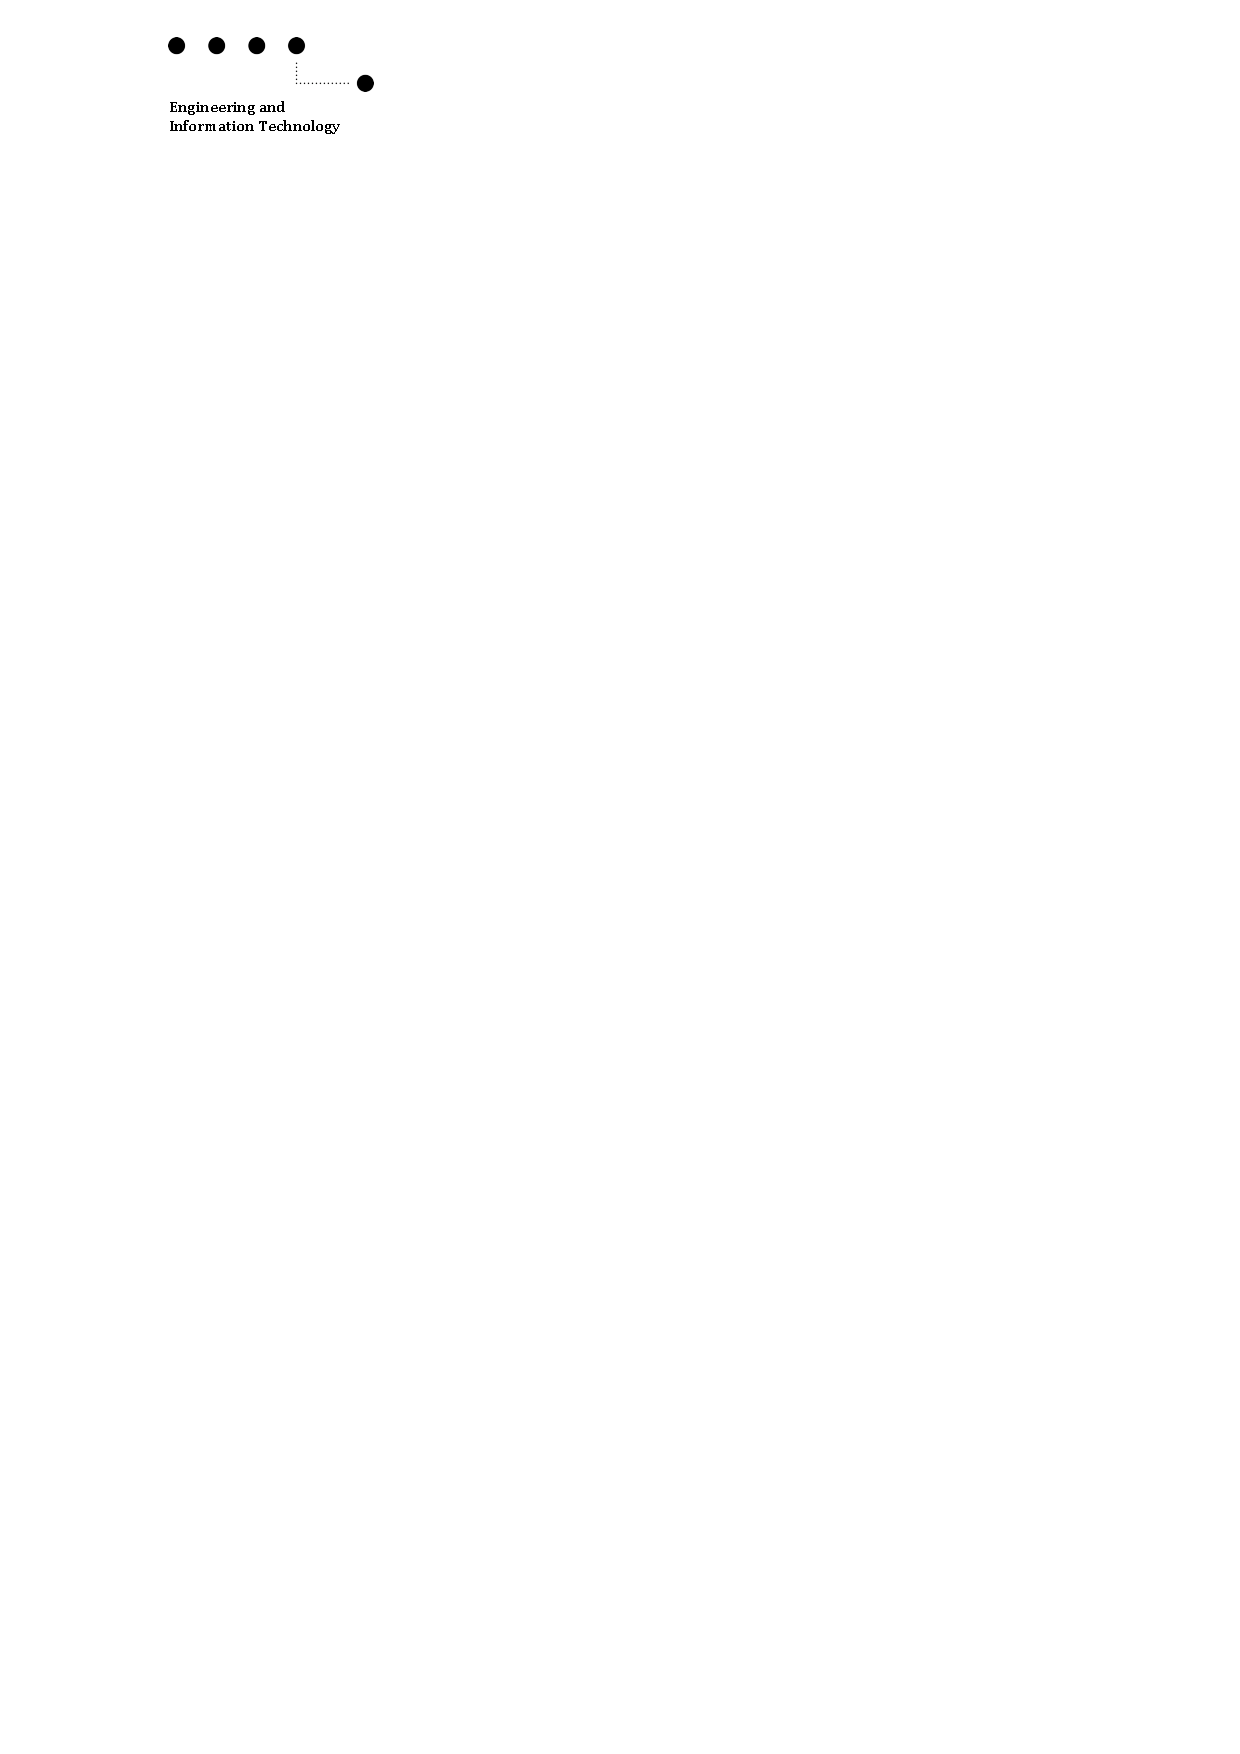
\includegraphics[height=3.5\baselineskip]{../figures/header}}
\fancyhead[RO, LE]{\leftmark}
%\fancyhead[CE]{\sectfont\bfseries \thechapter. Kapitel}
\fancyfoot[LE,RO]{\small \thepage}
\pagestyle{fancy}

 
\addtolength{\headheight}{2.2\baselineskip} 
%\addtolength{\headheight}{0.61pt}

\fancypagestyle{plain}{%
% head

\fancyhead[RE,LO]{\small \sectfont\bfseries 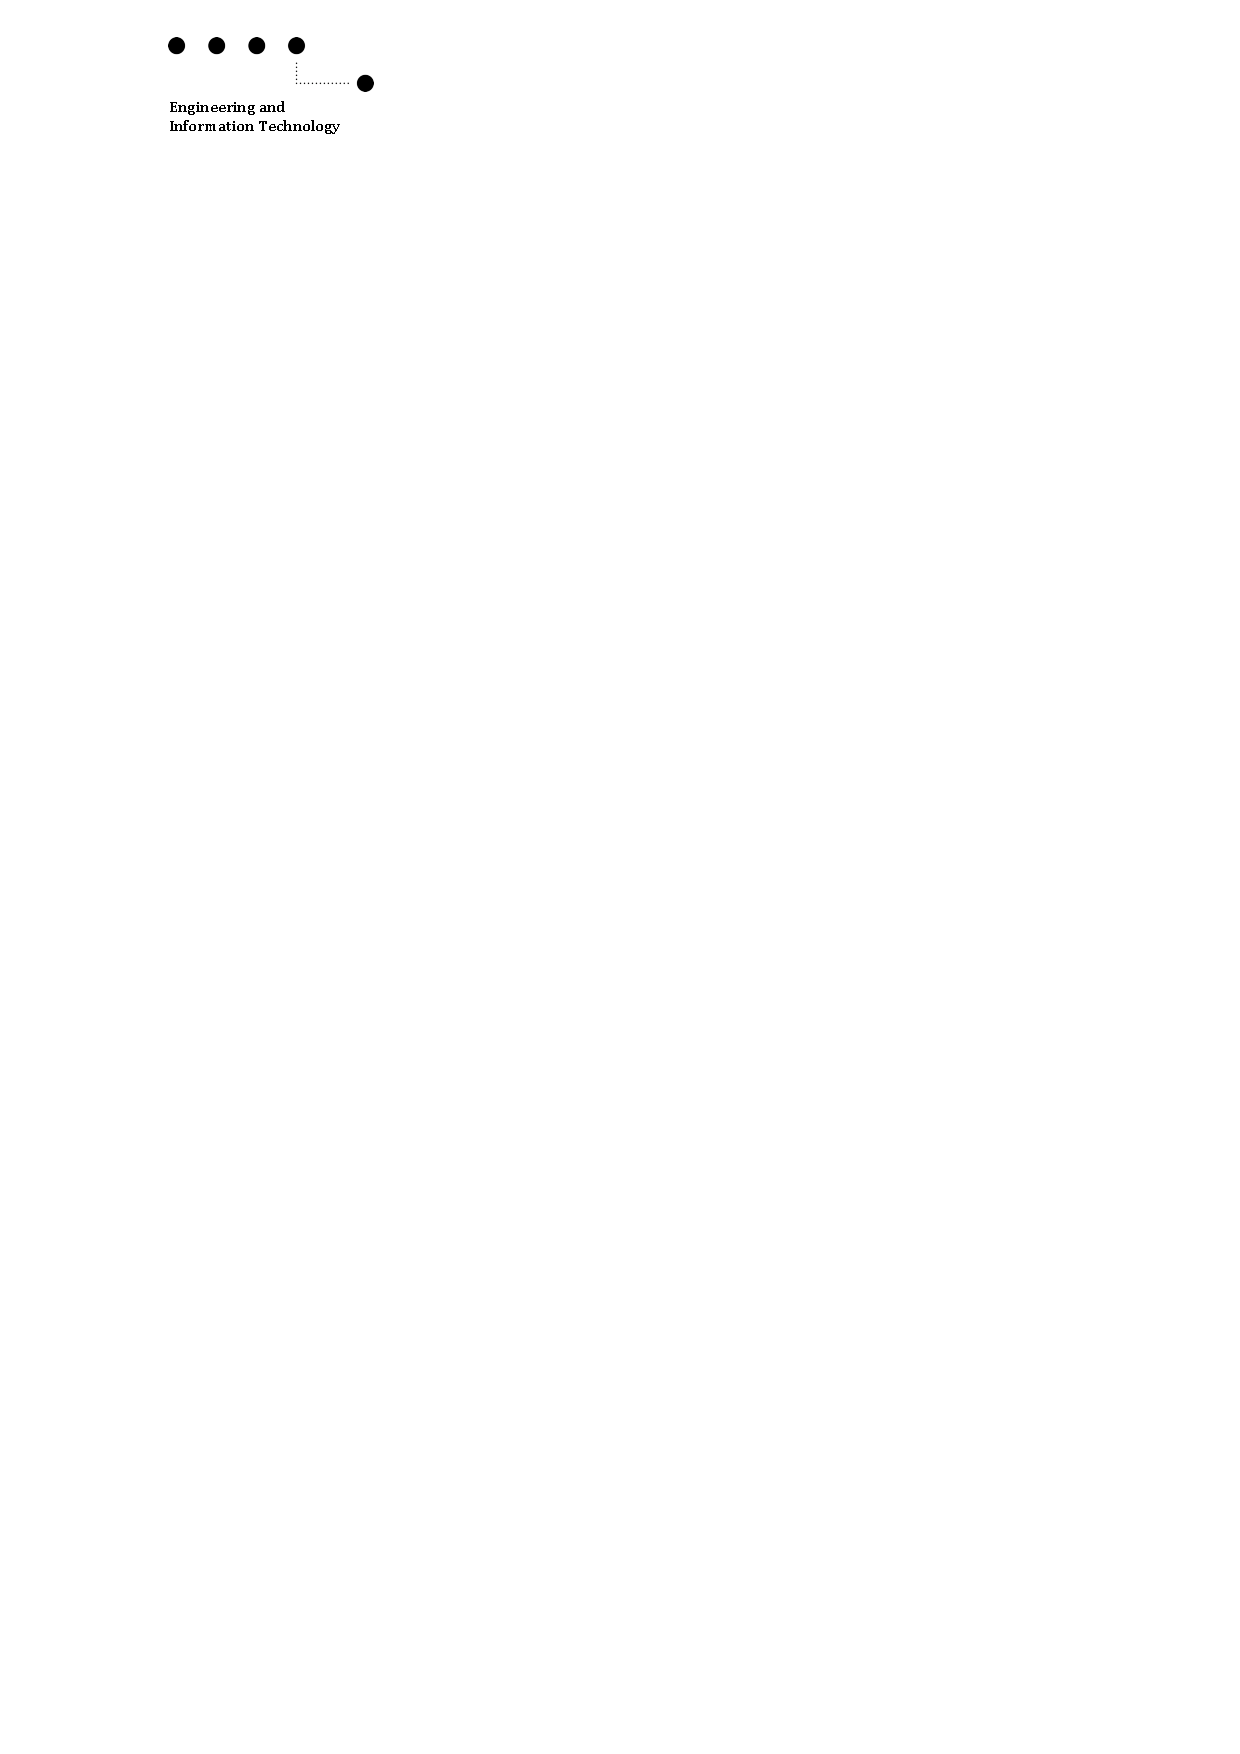
\includegraphics[height=3.5\baselineskip]{../figures/header}}
\fancyhead[RO,LE]{\leftmark}
%\fancyhead[CE]{\sectfont\bfseries \thechapter. Kapitel}
\fancyfoot[LE,RO]{\small \thepage}
\pagestyle{fancy}
}

\begin{document}
	
\begin{titlepage}
 
\begin{flushleft}

\vspace*{-2in}
\includegraphics[scale=1.1]{../tex-include/figures/title_header}

\vspace*{2in}

\begin{tabular}{p{5cm}p{8cm}}
\Large{Bachelor Thesis} & \Large{2009} \\ 
\end{tabular}

\vspace{1.8cm}
\begin{tabular}{ll}
\Huge{\bfseries CAVE Rendering Framework}\\[0.3cm]
\huge{User Manual}\\[1.8cm]
\end{tabular}

\begin{tabular}{p{5cm}p{8cm}}
\Large{Division} & \Large{CPVR}\\[0.2cm]
\Large{Authors} & \Large{Brigitte Hulliger}\\[0.2cm]
& \Large{Jonas Walti}\\[0.2cm]
& \Large{Stefan Broder}\\[0.2cm]
\Large{Supervisors} & \Large{Prof. U. K\"unzler} \\[0.2cm]
& \Large{Michael Luggen }\\[0.2cm]
& \\[0.2cm]
\Large{Version} & \Large{1.0}\\
\end{tabular} 

 \end{flushleft}
\end{titlepage}

\pagebreak
%\Large{\bfseries History}
\begin{table}
	\centering
	\begin{tabular}{|p{0.15\textwidth}|p{0.1\textwidth}|p{0.2\textwidth}|p{0.4\textwidth}|}
		\hline
		\bfseries Date & \bfseries Version & \bfseries Name & \bfseries Comment \\
		\hline
		\hline 05.06.2009 & 0.8 & all & First draft for expert H. van der Kleij \\
		\hline 09.06.2009 & 0.9 & all & Draft for Supervisors \\
		\hline 12.06.2009 & 1.0 & all & Last corrections for delivery \\
		\hline
	\end{tabular}
	\caption{History}
\end{table}
\pagebreak

\pagenumbering{roman}

\newacronym{bfhti}{BFH-TI}{Berner Fachhochschule - Technik und Informatik}
\newacronym{cpvr}{CPVR}{Computer Perception \& Virtual Reality}
\newacronym{cave}{CAVE}{Cave Automatic Virtual Environment}
\newacronym{vr}{VR}{Virtual Reality}
\newacronym{osg}{OSG}{OpenSceneGraph}
\newacronym{crf}{CRF}{CAVE Rendering Framework}
\newacronym{vrml}{VRML}{Virtual Reality Modeling Language}
\newacronym{x3d}{X3D}{}
\newacronym{opengl}{OpenGL}{Open Graphics Library}
\newacronym{glsl}{GLSL}{GL Shading Language}
\newacronym{api}{API}{Application Programming Interface}
\newacronym{ogre}{OGRE}{Object-Oriented Graphics Rendering Engine}
\newacronym{bof}{BOF}{Birds-Of-a-Feather}
\newacronym{cpu}{CPU}{central processing unit}
\newacronym{gpu}{GPU}{graphics processing unit}
\newacronym{fps}{fps}{framerate per second}
\newacronym{ascii}{ASCII}{American Standard Code for Information Interchange}
\newacronym{ssh}{SSH}{Secure Shell}
\newacronym{oo}{OO}{Object Oriented}
\newacronym{lgpl}{LGPL}{GNU Lesser General Public License}


% Inhaltsverzeichnis
\tableofcontents

% Abbildungsverzeichnis
\listoffigures

% Tabellenverzeichnis
\listoftables

% Listings 
\lstlistoflistings

\newpage
\pagenumbering{arabic}

% =======================================
% User Manual
% =======================================
\chapter{User Guide}
% Introduction - hullb2
% ==========================================
% Thesis Report - Introduction ( brods1 )
% ==========================================

\chapter{Introduction}
Over the past sixteen weeks we worked on a project within the scope of our bachelor thesis. The thesis report shows the reader what we made when we began and how we organised ourselves. Furthermore, we bring up what preparation work needed to be done, how we advanced during the project and how we tested our results. Finally, we point out unachieved goals and summarise an outlook on what could be done in the future.


% Installation - hullb2
% ==========================================
% User Manual - Installation ( hullb2/waltj3 )
% ==========================================
\section{Installation}

The CRF was tested on two setups:

\begin{itemize}
	\item \nameref{sec:ubuntu_setup}
	\item \nameref{sec:win_setup}
\end{itemize}

There are several dependencies you have to be aware of in order to setup a proper environment. Both setups have their own dependencies. They are all listed and described below.

\subsection{Linux Ubuntu 8.10}
\label{sec:ubuntu_setup}

We assume that you already have a running Ubuntu on your machine. Make sure you have the correct graphics drivers installed (i.e. nvidia-glx-dev for nvidia graphics cards). It is mandatory that you have the developer drivers installed (not the nvidia-glx only), because the CRF must be able to reference the header files. The CRF requires a running CMake, \gls{osg} and Equalizer setup.

\subsubsection{CMake}
\begin{table}[H]
	\centering
	\begin{tabular}{|p{0.2\textwidth}|p{0.75\textwidth}|}
		\hline Download & \href{http://www.cmake.org}{http://www.cmake.org} \\
		\hline Minimal Version & CMake 2.6 \\
		\hline Documentation & \href{http://cmake.org/cmake/help/documentation.html}{http://cmake.org/cmake/help/documentation.html} \\
		\hline
	\end{tabular}
	\caption{CMake Installation}
\end{table}

The CRF as well as OSG requires CMake. To install CMake on Ubuntu, you simply have to run the following command in a terminal:

\begin{lstlisting}[language=bash,caption={Install cmake on Ubuntu}]
% sudo apt-get install cmake
\end{lstlisting}

To install CMake on other Linux distributions you can compile it from source. The instructions can be found online.

\subsubsection{OSG}
\begin{table}[H]
	\centering
	\begin{tabular}{|p{0.2\textwidth}|p{0.75\textwidth}|}
		\hline Download & \href{http://www.openscenegraph.org/projects/osg/wiki/Downloads}{http://www.openscenegraph.org/projects/osg/wiki/Downloads} \\
		\hline Minimal Version & OSG 2.8 \\
		\hline Documentation & \href{http://www.openscenegraph.org/projects/osg/wiki/Support}{http://www.openscenegraph.org/projects/osg/wiki/Support} \\
		\hline
	\end{tabular}
	\caption{OSG Installation}
\end{table}

It is currently not possible to install OSG as simple as CMake on Ubuntu since aptitude only includes OSG-2.2 which is too old for the CRF. Therefore, make sure you install OSG from source. 
OSG requires some libraries which have to be installed on the system before you can start compiling OSG itself. Make sure you have the following packages installed on your system:

\begin{table}[H]
\centering
\begin{tabular}{|l|l|l|}
\hline \bfseries fileformat & \bfseries unix library  & \bfseries ubuntu package \\ 
\hline
\hline  tiff imges & libtiff & libtiff*-dev \\
\hline  jpeg images & libjpeg &  \\
\hline  gif images & libungif & \\
\hline  png images & libpng & libpng*-dev \\
\hline  true type fonts & freetype & libfreetype*-dev \\
\hline  libcurl & libcurl & libcurl4-openssl-dev \\
\hline  mesa & libmesa & mesa-common-dev \\
\hline  freeglut & libglut & freeglut-dev \\
\hline
\end{tabular} 
\caption{Dependencies for OSG}
\end{table}

Assuming you have gone through all prerequisists you can install OSG itself now.
We suggest that you use the following file structure on \textit{all} your workstations to ensure a proper setup. The CD attached provided with this manual contains an archive file \texttt{crf.zip}. This archive contains the source code of OSG as well as any needed data files. Copy the directory to your home directory:

\begin{lstlisting}[language=bash,caption={CRF installation}]
% cp crf.zip ~/
% unzip crf.zip
\end{lstlisting}

If you have a proper CMake setup and all required libraries, you should be able to run \texttt{configure} and get a similar result as listed below:

\begin{lstlisting}[language=bash,caption={OSG configuration}]
% cd ~/crf/OSG-2.8/
% ./configure
[...]
The build system is configured to instal libraries to /usr/local/lib
Your applications may not be able to find your installed libraries unless you:
    set your LD_LIBRARY_PATH (user specific) or
    update your ld.so configuration (system wide)
You have an ld.so.conf.d directory on your system, so if you wish to ensure that
applications find the installed osg libraries, system wide, you could install a
OSG specific ld.so configuration with:
    sudo make install_ld_conf

-- Configuring done
-- Generating done

% sudo make install_ld_conf
\end{lstlisting}

If \texttt{configure} doesn't work or gets a different result than the one above, make sure you correct the errors before you advance. You can save yourself a lot of time! \\

To install OSG, simply run \texttt{make} as user:
\begin{lstlisting}[language=bash,caption={OSG installation}]
% make
\end{lstlisting}

The installation of OSG may take up to two hours, depending on your hardware. So don't hesitate to get yourself a coffee now...

Assuming a proper \texttt{make}, run \texttt{make install} as root:

\begin{lstlisting}[language=bash,caption={Finish OSG installation}]
% sudo make install
\end{lstlisting}

This copies the OSG libraries to the right directories on your system.

\paragraph{Setting System Variables}\hfill\\
To finish your OSG setup you have to set some system variables. To do so, edit your \texttt{/etc/environments} as root. Add the following line to this file:

\begin{lstlisting}[language=bash,caption={/etc/environment}]
OSG_FILE_PATH=/home/<user>/crf/OSG-Data
\end{lstlisting}


\subsubsection{Equalizer}

\begin{table}[H]
	\centering
	\begin{tabular}{|p{0.2\textwidth}|p{0.75\textwidth}|}
		\hline Download & \href{http://www.equalizergraphics.com/downloads/major.html}{http://www.equalizergraphics.com/downloads/major.html} \\
		\hline Minimal Version & Equalizer 0.6 \\
		\hline Documentation & \href{http://www.equalizergraphics.com/documents/EqualizerGuide.pdf}{http://www.equalizergraphics.com/documents/EqualizerGuide.pdf} \\
		\hline
	\end{tabular}
	\caption{Equalizer Installation}
\end{table}

Equalizer has to be installed from source too. Before you start compiling it, make sure you have installed the following packages on your system:

\begin{table}[H]
\centering
\begin{tabular}{|l|l|l|}
\hline \bfseries unix library  & \bfseries ubuntu package \\ 
\hline
\hline  bison & bison \\ 
\hline  flex & flex  \\ 
\hline  libuuid & e2fsprogs  \\
\hline
\end{tabular} 
\caption{Dependencies for Equalizer}
\end{table}

After installing the prerequisits, simply run \texttt{make} and \texttt{make install} in the source folder of Equalizer: 

\begin{lstlisting}[language=bash,caption={Equalizer installation}]
% cd ~/crf/equalizer-0.6-rc1/
% make
% sudo make install
\end{lstlisting}

You can simply test your Equalizer installation by running the sample application \texttt{eqPly}, which is the sample application provided by Equalizer:

\begin{lstlisting}[language=bash,caption={Test Equalizer by example application eqPly}]
% cd /usr/local/bin
% eqPly
\end{lstlisting}

A screenshot of the expected output of the \texttt{eqPly} and the \texttt{eVolve} application is attached in Appendix \ref{sec:eqSample}.

\subsubsection{SSH Setup}
In order to use Equalizer on a distributed setup with multiple rendering clients, each client as well as the server necessarily have to run a SSH server. The server must be able to connect to each client without entering a passwort. Analogously, each client must be able to connect to the server. The easiest way to achieve this is using public key authentication. This can be set up as follows.

Step 1: If not already done, we have to create a key pair (public and private key) on each component:
\begin{lstlisting}[language=bash,caption={SSH Key generation}]
% ssh-keygen
Generating public/private rsa key pair.
Enter file in which to save the key (/home/stefan/.ssh/id_rsa):
% <enter>
Enter passphrase (empty for no passphrase):
% <enter>
Enter same passphrase again:
% <enter>
\end{lstlisting}
We want neither to store the keys somewhere other than in the default directory nor want we to enter a passphrase. Therefore, just press <enter> without typing anything. In this case, we just care about the connection, not so much about the security provided by SSH.

Step 2: Now, the public key has to be added to the authorized\_keys file on each node we want to connect to. Remember that this proceedings have to be done for both directions, from the node running the eqServer to each client and vice versa.
\begin{lstlisting}[language=bash,caption={RSA-Key distribution}]
% scp ~/.ssh/id_rsa.pub <ip-of-host>:/home/<username>
# enter password
% ssh <ip-of-host> "cat id_rsa.pub >> ~/.ssh/authorized_keys && rm id_rsa.pub"
# enter password again
\end{lstlisting}

If everything worked fine, then you should be able to connect without entering a password from now on. If not, go back to the last step and ensure you followed consequently. To test the connection enter
\begin{lstlisting}[language=bash]
% ssh <ip-of-host> 
\end{lstlisting}


\subsubsection{CRF}

Change to the CRF directory where the CMakeLists.txt file resides. There, type the following commands.

\begin{lstlisting}[language=bash,caption={CRF installation}]
% cmake .
% make
% sudo make install
\end{lstlisting}

If you experience any errors after the \texttt{cmake} command, you most probably forgot to follow one of the previous instructions. Otherwise, you installed the CRF on you system. If you use a distributed system with multiple clients, you can distribute the binaries and header files using the shell script distributed with the sources.

Be careful, if you want to use debug libraries. To do so, tell CMake by setting the SET\_DEBUG\_LIBS variable: \texttt{SET( USE\_DEBUG\_LIBS ON )}. Verify that CMake did choose the correct libraries (libnames of \gls{osg} end with d for debug). Be consistent, take eiter the debug libraries from both, \gls{osg} and Equalizer, or from none. This can be done using \texttt{ccmake}.


\subsection{Windows XP}
\label{sec:win_setup}

In order to install the CRF, you a build environment (e.g. Ms Visual C++). Furthermore, it is expected that you have installed the OpenGL library and header files. In the following, we guide you through the installation of CMake, OSG, Equalizer and, finally, the CRF.

\subsubsection{CMake}

\begin{table}[H]
	\centering
	\begin{tabular}{|p{0.2\textwidth}|p{0.75\textwidth}|}
		\hline Download & \href{http://www.cmake.org}{http://www.cmake.org} \\
		\hline Minimal Version & CMake 2.6 \\
		\hline Documentation & \href{http://cmake.org/cmake/help/documentation.html}{http://cmake.org/cmake/help/documentation.html} \\
		\hline
	\end{tabular}
	\caption{CMake Installation}
\end{table}

The CRF as well as OSG require CMake to be built. To install CMake on Windows XP, just visit the CMake and follow the install instructions. 

Generally, to build the desired project file for Visual C++ using CMake you most probably want to use the CMake GUI. Watch out for the CMakeLists.txt. Then, let CMake create the project files at the selected location.


\subsubsection{OSG}

\begin{table}[H]
	\centering
	\begin{tabular}{|p{0.2\textwidth}|p{0.75\textwidth}|}
		\hline Download & \href{http://www.openscenegraph.org/projects/osg/wiki/Downloads}{http://www.openscenegraph.org/projects/osg/wiki/Downloads} \\
		\hline Minimal Version & OSG 2.8 \\
		\hline Documentation & \href{http://www.openscenegraph.org/projects/osg/wiki/Support}{http://www.openscenegraph.org/projects/osg/wiki/Support} \\
		\hline
	\end{tabular}
	\caption{OSG Installation}
\end{table}

Visit the OSG website and look for the downloads section. Download the above mentioned version of OSG (this guide was tested with 2.8.0 and 2.8.1). You can either simply download and install the binaries or download the source code and compile it by yourself. Just be warned, compile OSG can take up to two hours. Verify that you have fulfill all the requirements mentioned on the website. Now, unpack the zip archive.

If you have chosen to compile OSG by yourself, then go for it and compile it. In any case, you should install the OSG on your system. Make shure to set the path of the OSG data files in the PATH environment variable.

\subsubsection{Equalizer}
\begin{table}[H]
	\centering
	\begin{tabular}{|p{0.2\textwidth}|p{0.75\textwidth}|}
		\hline Download & \href{http://www.equalizergraphics.com/downloads/major.html}{http://www.equalizergraphics.com/downloads/major.html} \\
		\hline Minimal Version & Equalizer 0.6 \\
		\hline Documentation & \href{http://www.equalizergraphics.com/documents/EqualizerGuide.pdf}{http://www.equalizergraphics.com/documents/EqualizerGuide.pdf} \\
		\hline
	\end{tabular}
	\caption{Equalizer Installation}
\end{table}

If you use Equalizer with Windows you have to change a line in the Equalizer 0.6 sources, before compiling. In the Equalizer file   \texttt{src/lib/client/event.h} you need to add \texttt{EQ\_EXPORT} in front of the default constructor of the \texttt{Event} struct to make this constructor visible for the Equalizer.dll users (like the \gls{crf}). This change will be integrated in further Equalizer releases. 

Now the source is ready to compile.


\subsubsection{SSH Setup}

In order to use Equalizer on a distributed setup with multiple rendering clients, you must run a SSH server on every client. This scenario was not tested with Windows clients. My suggestion is to emulate a linux using Cygwin\footnote{http://www.cygwin.com/} or equivalent. If you want to try, install Cygwin and continue with the "SSH Setup" chapter of Ubuntu. Again, this was not tested, so you are on your own here.

\subsubsection{CRF}

Finally, you should be able to install the CRF. Unzip the crf archive, use CMake to generate the project files, build and install it. Now you can take full advantage of the CRF. 

Be careful, if you want to use debug libraries. To do so, tell CMake by setting the SET\_DEBUG\_LIBS variable: \texttt{SET( USE\_DEBUG\_LIBS ON )}. Verify that CMake did choose the correct libraries (libnames of \gls{osg} end with d for debug). Be consistent, take eiter the debug libraries from both, \gls{osg} and Equalizer, or from none. This can be done using the CMake GUI.


\chapter{Programming Guide}
% Example - waltj3
% ==========================================
% User Manual - Example ( all )
% ==========================================
\section{Overview}
This section shows how the \gls{crf} can be used. This is achieved by showing some examples in a tutorial style. There are also some special features described here. To get a better overview of the used techniques, please consider the Technical Report. For an overview of all classes with its functions, take a look at the provided \gls{api}.
The base classes of the \texttt{eqOsg} and the \texttt{crf} namespaces provide some basic functionality. When overriding the functions of theses classes, be careful not to lose a desired functionality. It is often useful and sometimes a must to call the original function of the base class in your reimplementation. 
To avoid already known errors, please consult the \emph{Technical Report} (especially the \emph{Limitations} section).

\section{Prerequisites}
\label{sec:Prerequisites}
All the following examples require a correct and complete installation of Equalizer, \gls{osg} and the \gls{crf} with well set environment variables and all necessary files available. 

\section{World Coordinate System}
\label{sec:WorldCoordinateSystem}
The coordinate system of Equalizer, used in all the Equalizer demo-applications and for the head transform matrix of Equalizer, differs from the one of \gls{osg}. \gls{osg} uses the z-axis as up-vector. In contrast, Equalizer uses the y-axis as up-vector. Therefore in Equalizer, the z-axis points away from the user. This is well known as left-handed system. To convert the \gls{osg} world coordinate system to the one of Equalizer, just use \texttt{eqOsg::Pipe::correctCoordSys(yourRootNode)} to rotate the scene graph. This function rotates the passed node 90� around the x-axis and 180� around the y-axis and returns the converted node. 

The conversion to the behaviour of Equalizer makes it easier for further framework extensions like tracker support or similar. 
 
\section{Global Keystrokes}
If none of the \texttt{eqOsg} event related functions are overridden (like in the following HelloWorld examples) there are several key bound actions available:
\subsubsection{General Keys}
\label{sec:GeneralKeys}
\begin{itemize}
	\item F2: toggle through the \gls{osg} overlay statistics (consider the \gls{osg} documentation \cite{osgGuide} for further information)
	\item F3: enable/disable the Equalizer camera handling
	\item F4: enable/disable the \gls{crf} framerate counter
	\item F5: enable/disable the Equalizer drawing statistics (consider the  Equalizer Programming Guide \cite{eqPG} for further information )
	\item F6: enable/disable the bottom-left info text
\end{itemize}

\subsubsection{Camera Handling}
\label{sec:CameraHandling}
There is a basic FPS\footnote{FPS - First Person Shooter: A video game genre with a common and well known camera controlling behaviour. The head is rotated by the mouse and the movement is done with keys.}-like camera built in. 
\begin{itemize}
	\item w, Up-Arrow: move along the z-axis (forward)
	\item s, Down-Arrow: move along the z-axis (backward)
	\item a, Left-Arrow: move along the x-axis (to the left)
	\item d, Right-Arrow: move along the x-axis (to the right)
	\item Page-Up: move along the y-axis (upwards)
	\item Page-Down: move along the y-axis (downwards)
	\item Left-Mouse-Button \& Mouse Movement: rotate the local coordinate system of the camera, thus its view matrix (all the above described axes do change accordingly, similar to navigate an aircraft)
\end{itemize}

\section{HelloWorld}
The most simple \gls{crf} application can be realised by these lines of code:

\begin{lstlisting}
{
#include <crf/crfStarter.h>

//1. Create the main method, which calls the crfStart.run()
//method to start Equalizer and stuff
int main(int argc, char** argv) 
	
	//create the CRF starter
	crf::crfStarter starter;

	//run the application
	starter.run(argc,argv);
}
\end{lstlisting}
To run this example with a custom Equalizer topology, start your Equalizer server with the desired configuration file. If multiple nodes are used, make sure that on every machine the HelloWorld application and all the \gls{osg} files are placed in the same directory.

\begin{figure}[H]
	\centering
		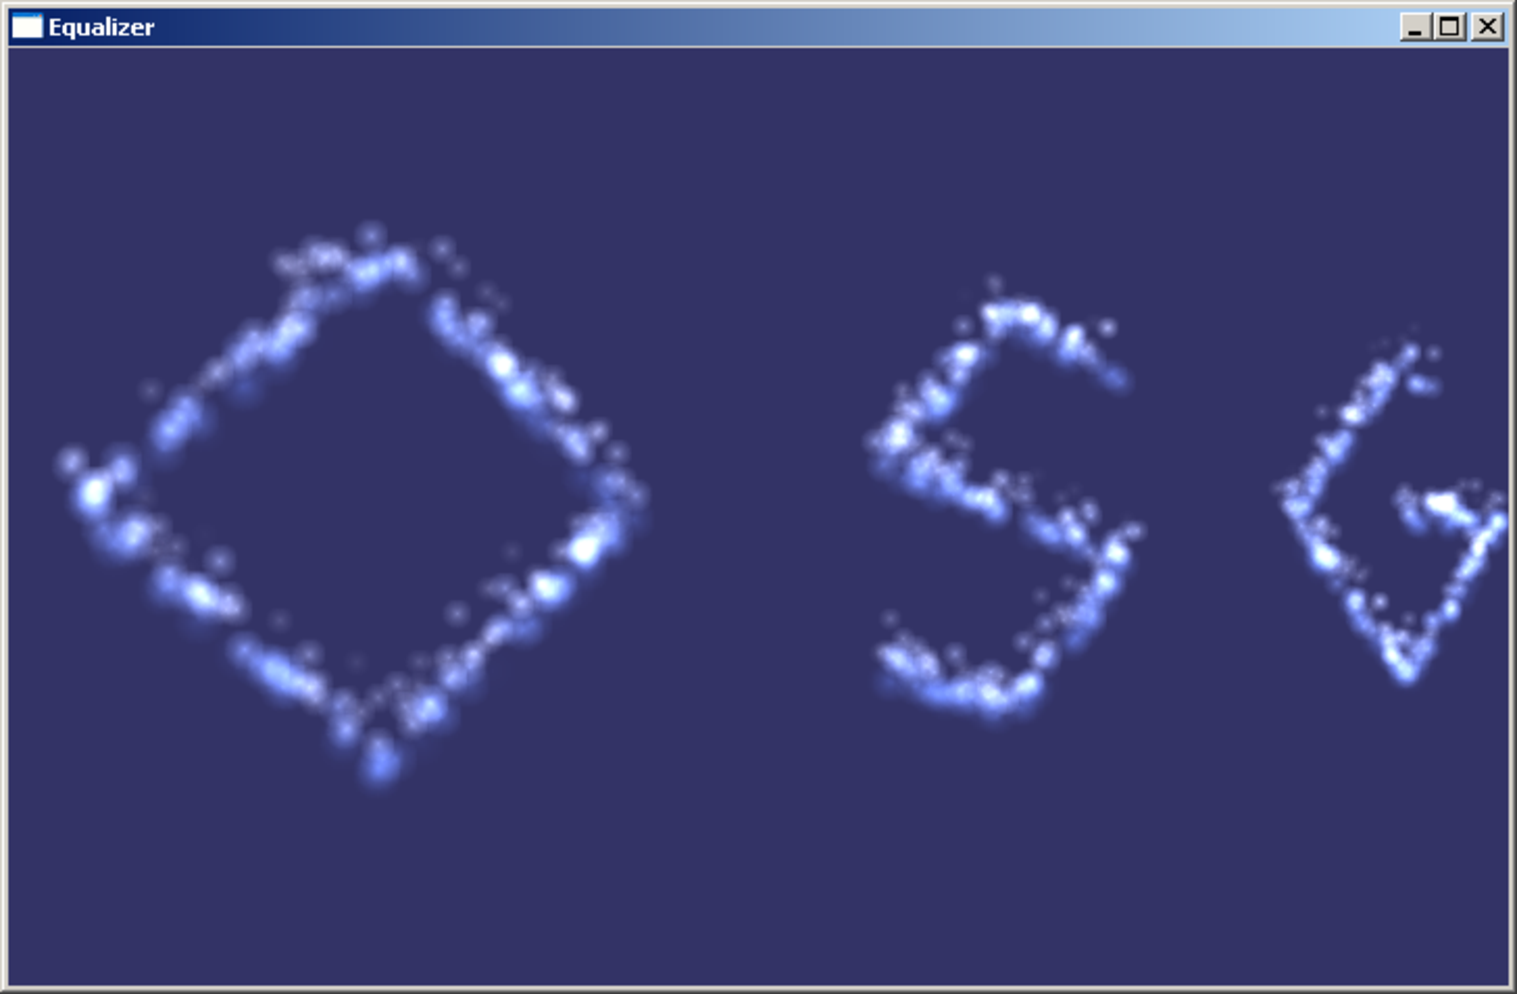
\includegraphics[width=0.6\textwidth]{../figures/pg_ex1_scr1}
	\caption{HelloWorld output with the standard Equalizer configuration}
	\label{fig:pg_ex1_scr1}
\end{figure}


\subsubsection{Background Information}
\label{sec:BackgroundInformation}
Why does this work? The crfStarter class is a fa�ade which initialises the whole Equalizer application. Thereafter, the default functions of the framework are called and if the environment variable \texttt{OSG\_FILE\_PATH} is set and the OSG file \texttt{osgcool.osg} is available there, a simple animated text ``OSG'' should appear on the screen(s). If this works, your parallel rendering system with Equalizer and \gls{osg} is set up correctly and you are able to continue.

\section{Loading OSG Models}
\label{sec:LoadingOSGModels}
With a working HelloWorld example, you are now able to load any \texttt{.osg} file into this \gls{crf} application. To do this, run your compiled and fully linked HelloWorld example with the \texttt{--model=<filename>.osg} argument. Make sure that this model is available on every node in the same directory.

IMPORTANT: Several segmentation faults occurred when trying to use \texttt{osgDB::readNodeFile()} (like in the HelloWorld example) with multipipe configurations and just one running instance of the application. This is because \texttt{osgDB::readNodeFile()} messes up memory when executed multiple times. Therefore, we introduced a mechanism which does load the model just once and shares it with the different \gls{osg} viewers on the same machine (use the \texttt{--mode=pipesafe} argument when starting the shipped crfHelloWorld application). This did not accuron on multinode configurations with just one running instance per pipe.

\subsubsection{Windows Example}
\label{sec:WindowsExample}

To start the application with a desired model:

\begin{lstlisting}
c:\HelloWorld\>HelloWorld.exe --model=cow.osg
\end{lstlisting}

\begin{figure}[H]
	\centering
		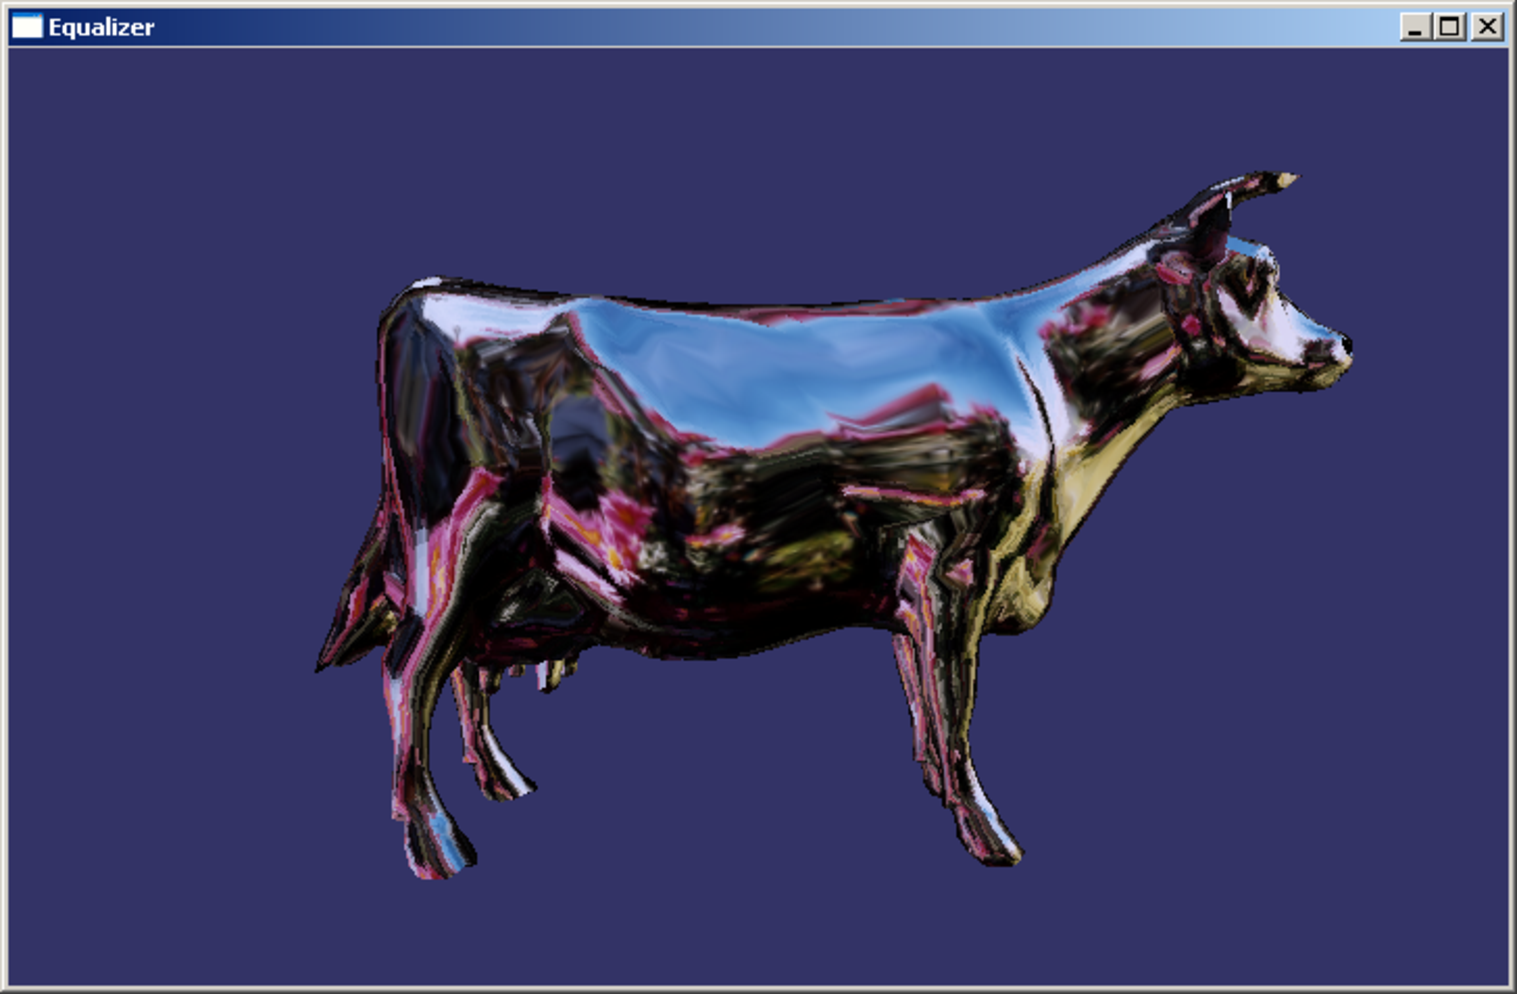
\includegraphics[width=0.6\textwidth]{../figures/pg_ex2_scr1}
	\caption{HelloWorld output with a model as command line argument}
	\label{fig:pg_ex2_scr1}
\end{figure}

\section{Custom Scene Graph}

To use the whole power of the \gls{crf} and to create animated and dynamic scene graphs, the following steps have to be realised:
\begin{enumerate}
	\item create your own pipe class, inherited from the \texttt{crfPipe} class
	\item override desired functions like \texttt{createSceneGraph}, \texttt{updateSceneGraph} or others
	\item create your own factory class which returns your custom objects, based on \texttt{crfNodeFactory}
	\item pass your factory instance to the \texttt{crfStarter} using \texttt{crfStarter::setNodeFactory(yourFactory)} function
	\item run the application with the \texttt{crfStarter.run} function
\end{enumerate}

With this approach, the \gls{crf} user is able to override a lot of functions and therefore customise his \gls{crf} application. The following examples should provide an overview of some of the possibilities. To get a complete survey, consider the \gls{api} and the Technical Documentation of the \gls{crf} and Equalizer.

\section{Scene Graph Creation}

A common way for creating custom scene graphs is:

\begin{enumerate}
	\item Create a class with all your behaviours of your scene graph. This class provides a \texttt{getScene()} function which returns the root node of your scene graph.
	\item in your custom \texttt{createSceneGraph()} function, add this root node to the \gls{osg} \texttt{\_viewer->setSceneData(mySceneGraph->getScene())}
\end{enumerate}

\section{Animated Scenes}

\subsubsection{Example 1}
\label{sec:Example1}
To create an animation for your scene graph, a common CRF approach would be:

\begin{enumerate}
	\item override the \texttt{crfPipe::updateSceneGraph} function to call the update function of your scene graph
\end{enumerate}

\begin{lstlisting}[caption={calling the updated function of your scene graph}]
void crfDemoApp::Pipe::updateSceneGraph(){
 //call the univers' update function
 myUniverse->update(getConfig()->getTime());
}
\end{lstlisting}

Note: \texttt{GetConfig()->getTime()} calls the synchronous Equalizer time.

\subsubsection{Example 2}
\label{sec:Example2}

A more straight-forward approach:

\begin{enumerate}
	\item create a new member for the animation in your pipe class (a rotation node e.g.)
	\item attach this node to your scene graph in your \texttt{createSceneGraph} implementation
	\item attach the to-rotate-node to this rotation node
	\item update this node in \texttt{updateSceneGraph()}
\end{enumerate}

The \texttt{updateSceneGraph()} function gets called every time a new frame is drawn. As one can see, the  \texttt{config->getTime()} function of Equalizer is used to rotate framerate independently. One could also use the  \texttt{elapsedTime()} function provided by the \gls{osg} viewer but in that case, the time has to be reset when the first frame is drawn, because it is not granted that every clock of the \gls{osg} viewer starts at the same time in multinode and/or multipipe configurations. Remember: Every pipe has its completely independent \gls{osg} viewer!

\begin{lstlisting}[caption={the update function}]
void crfDemoApp::Pipe::updateSceneGraph(){
 osg::Matrix rotation = _rotateMatrix->getMatrix();
 rotation.makeRotate(getConfig()->getTime()*0.0024, osg::Vec3( 0., 0., 1. ) );
 _rotateMatrix->setMatrix(rotation);
}
\end{lstlisting}

\section{Example: Porting An OSG Application}
\subsection{Overview}
In order to give another example of the power of the \gls{crf}, we took the original \gls{osg} demo \texttt{osgkeyboard.cpp}, shipped with the \gls{osg} source code, and ported it to a fully functional \gls{crf} application. This example shows the ability of the \gls{crf} to handle common \gls{osg} based eventhandlers. Nothing has been changed in the eventhanlder class of this example. 

\subsection{Step 1: Small Example Changes}
To obtain a better structured application, we exported all the  class definitions of the \texttt{osgkeyboard.cpp} into a separate  header file named \texttt{keyboard.h}. Now we are able to use all the classes of the example by including just this header file. 
\subsection{Step 2: Building The CRF Application}
As mentioned before, we have to build up a more complex CRF application. To keep this demo simple, we do all this in the \texttt{main.cpp} file.
\begin{enumerate}
	\item necessary inlcudes \& namespaces:
	\begin{lstlisting}[caption={setting up the include directives}]
#include <crf/crfPipe.h>
#include <crf/crfNodeFactory.h>
#include <crf/crfStarter.h>

#include "keyboard.h"

using namespace osg;
using namespace std;
	\end{lstlisting}
	\item define a namespace and declare our custom pipe and node factory classes:
	\begin{lstlisting}[caption={declaring the custom classes}]
///to avoid conflicts with naming, create a own namespace for the concrete demo
namespace crfDemoApp {

///we create our own pipe by inheriting from the crfPipe
class Pipe : public crf::crfPipe {
  public:
      Pipe(eq::Node* parent) : crf::crfPipe(parent){
        _sceneGraphCreated=false;
      }
    protected:
      ///Our own method to create the scene graph
      void createSceneGraph();
};

///Create a custom-nodefactory to create our own custom pipe-object
class NodeFactory : public crf::crfNodeFactory {
  protected:
    virtual eq::Pipe* createPipe(eq::Node *parent){
    return new crfDemoApp::Pipe(parent);		
  }
};
\end{lstlisting}

\item Reimplement the \texttt{createSceneGraph()} function. The custom \gls{osg} eventhandler, implemented exactly as in the original \gls{osg} example, is linked to the viewer of the pipe. Thereafter, the rootnode of the keyboard is converted to the Equalizer coordinate system by passing the node to the \texttt{correctCoordsys()} function, which returns the node, rotated 90� around the x-axis and 180� around the y-axis to fit the commonly used coordinate system of Equalizer.
\begin{lstlisting}[caption={the createSceneGraph function}]
void crfDemoApp::Pipe::createSceneGraph(){
  osg::ref_ptr<keyboard::KeyboardModel> keyboardModel = new keyboard::KeyboardModel();

  _viewer->addEventHandler(new keyboard::KeyboardEventHandler(keyboardModel.get()));
  _viewer->setSceneData( correctCoordsys(keyboardModel->getScene()));

  _sceneGraphCreated=true;
}
\end{lstlisting}
\end{enumerate}
\subsection{Step 3: The Main Function}

\begin{enumerate}
	\item Create a \texttt{crfStarter} object, pass the custom factory and run the application.
\begin{lstlisting}[caption={the main function of the ported OSG example}]
int main(int argc, char** argv) 
{
  //create the demo factory
  crfDemoApp::NodeFactory* fac = new crfDemoApp::NodeFactory();
  
  //create the CRF starter
  crf::crfStarter starter;

  //pass the factory to the starter
  starter.setNodeFactory(fac);

  //run the application
  starter.run(argc,argv);
}
\end{lstlisting}
\end{enumerate}

\subsection{The Result}
\begin{figure}[h]
	\centering
		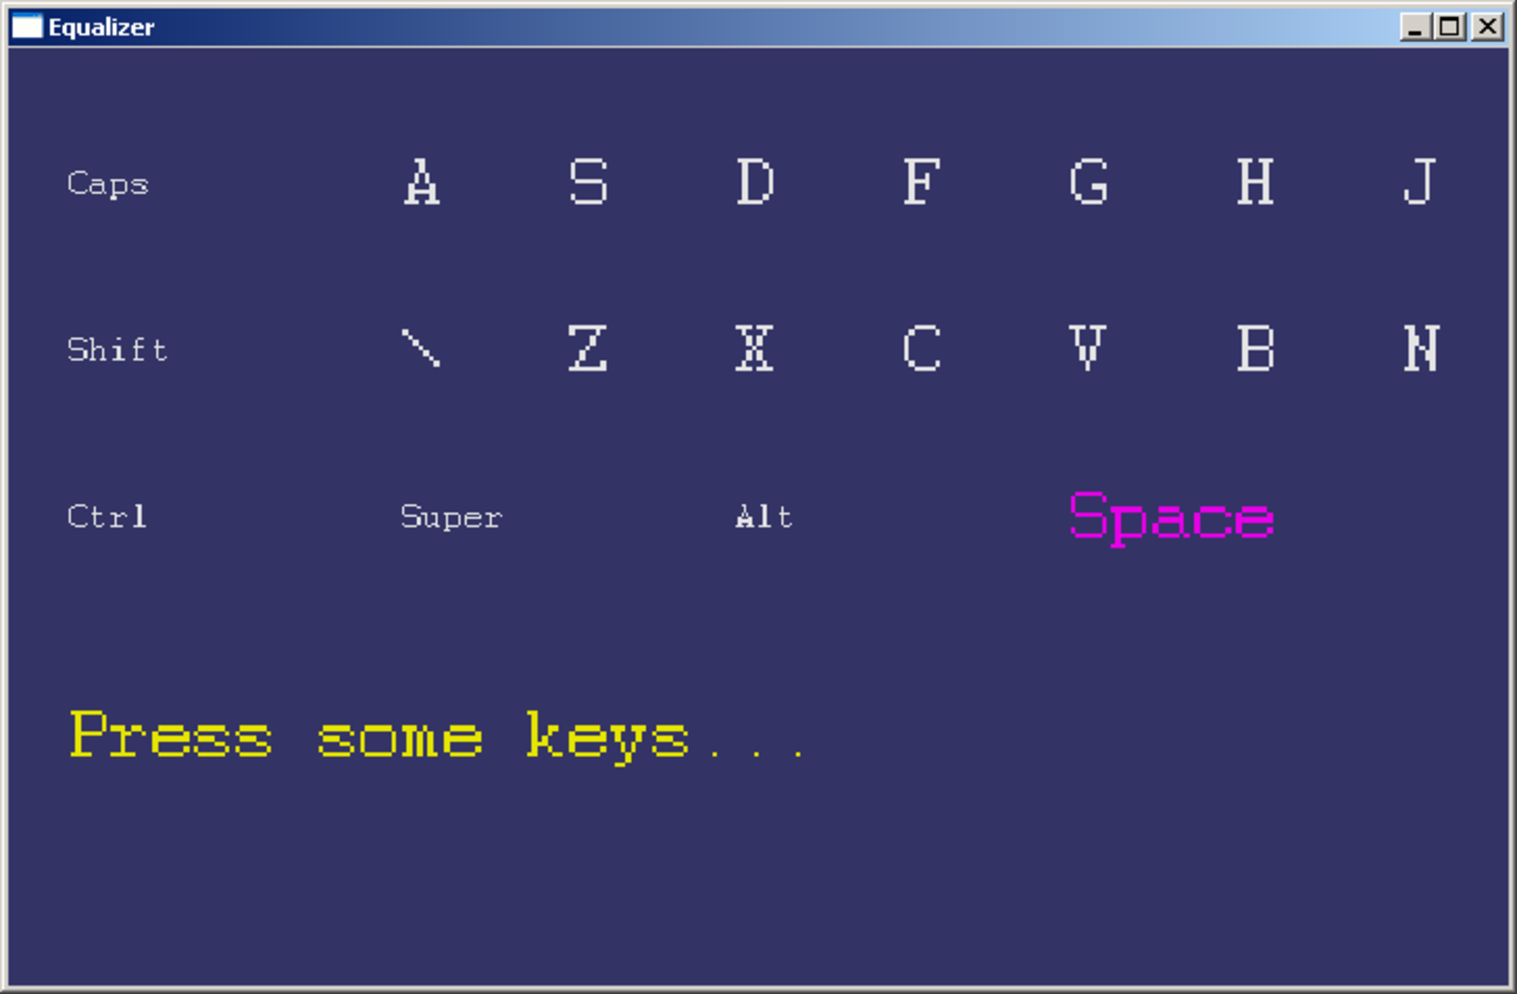
\includegraphics[width=0.60\textwidth]{../figures/pg_exKeyboard_scr1}
	\caption{screenshot of the ported OSG keyboard example}
	\label{fig:pg_exKeyboard_scr1}
\end{figure}

By the way: This example can easily be used to check which key events are passed to the OSG viewer, because the eventhandler highlights the pressed keys.






% =======================================
% Acronyms
% =======================================
\addcontentsline{toc}{chapter}{Glossary}
\printglossary[title={Glossary}]

% =======================================
% Bibliography
% =======================================
\addcontentsline{toc}{chapter}{Bibliography}
\bibliography{../tex-include/crfbibliography} % Note the lack of whitespace between the commas and the next bib file.

% =======================================
% Appendices
% =======================================
%\addcontentsline{toc}{chapter}{Appendices}
\appendix

\chapter{Worklog}
\label{sec:appendixWorklog}

\begin{table}[H]
	\centering
	\begin{tabular}{|b{0.1\textwidth}|p{0.3\textwidth}|p{0.1\textwidth}|p{0.1\textwidth}|p{0.23\textwidth}|}
		\hline \multicolumn{2}{|l|}{\color{red}{\bfseries 16.02.2009}} & \multicolumn{3}{l|}{\color{red}{\bfseries Project Start}} \\
		\hline
		\hline \bfseries week 1-2 & \multicolumn{4}{l|}{\bfseries 16.02.2009 - 26.02.2009} \\
		\hline
		\hline \bfseries who? & \bfseries what? & \bfseries output & \bfseries achieved & \bfseries comment \\ 
		\hline hullb2 & Equalizer knowledge & running Equalizer installation & \tick & \quad\quad- \\
		\hline waltj3 / brods1 & OSG/OGRE setup & \quad\quad- & \tick & \quad\quad- \\
		\hline all & index for requirement specification & \quad\quad- & \tick & \quad\quad- \\ 
		\hline
	\end{tabular}
	\caption{Worklog Week 1-2: 16.02.2009 - 26.02.2009}
\end{table}

\begin{table}[H]
	\centering
	\begin{tabular}{|b{0.1\textwidth}|p{0.3\textwidth}|p{0.1\textwidth}|p{0.1\textwidth}|p{0.23\textwidth}|}
		\hline \bfseries week 3 & \multicolumn{4}{l|}{\bfseries 27.02.2009 - 05.03.2009} \\
		\hline
		\hline \bfseries who? & \bfseries what? & \bfseries output & \bfseries achieved & \bfseries comment \\ 
		\hline all & Prototypes & \quad\quad- & \tick & \quad\quad- \\
		\hline all & eqOSG evaluation & \quad\quad- & \tick & \quad\quad- \\
		\hline all & eqOGRE evaluation & \quad\quad- & \tick & \quad\quad- \\
		\hline all & first draft of requirements specification & \quad\quad- & \tick & \quad\quad- \\
		\hline
	\end{tabular}
	\caption{Worklog Week 3: 27.02.2009 - 05.03.2009}
\end{table}

\begin{table}[H]
	\centering
	\begin{tabular}{|b{0.1\textwidth}|p{0.3\textwidth}|p{0.1\textwidth}|p{0.1\textwidth}|p{0.23\textwidth}|}
		\hline \bfseries week 4 & \multicolumn{4}{l|}{\bfseries 06.03.2009 - 12.03.2009} \\
		\hline
		\hline \bfseries who? & \bfseries what? & \bfseries output & \bfseries achieved & \bfseries comment \\ 
		\hline all & requirements specification finished & \quad\quad- & \tick & \quad\quad- \\
		\hline
		\hline all & \multicolumn{4}{l|}{\color{red}{\bfseries 13.03.09: Appointment with Expert: H. van der Kleij}} \\
		\hline
	\end{tabular}
	\caption{Worklog Week 4: 06.03.2009 - 12.03.2009}
\end{table}


\begin{table}[H]
	\centering
	\begin{tabular}{|b{0.1\textwidth}|p{0.3\textwidth}|p{0.1\textwidth}|p{0.1\textwidth}|p{0.23\textwidth}|}
		\hline \bfseries week 5 & \multicolumn{4}{l|}{\bfseries 13.03.2009 - 19.03.2009} \\
		\hline
		\hline \bfseries who? & \bfseries what? & \bfseries output & \bfseries achieved & \bfseries comment \\ 
		\hline all & corrections of requirements specification & \quad\quad- & \tick & \quad\quad- \\
		\hline
		\hline \color{red}{\bfseries M1} & \multicolumn{2}{l|}{\color{red}{\bfseries Functional specification}} & \tick & \quad\quad- \\
		\hline \color{red}{\bfseries M2} & \multicolumn{2}{l|}{\color{red}{\bfseries Prototype finished}} & \tick & \quad\quad- \\
		\hline
	\end{tabular}
	\caption{Worklog Week 5: 13.03.2009 - 19.03.2009}
\end{table}


\begin{table}[H]
	\centering
	\begin{tabular}{|b{0.1\textwidth}|p{0.3\textwidth}|p{0.1\textwidth}|p{0.1\textwidth}|p{0.23\textwidth}|}
		\hline \bfseries week 6 & \multicolumn{4}{l|}{\bfseries 20.03.2009 - 26.03.2009} \\
		\hline
		\hline \bfseries who? & \bfseries what? & \bfseries output & \bfseries achieved & \bfseries comment \\ 
		\hline all & Evaluate scene graph techniques & \quad\quad- & \tick & \quad\quad- \\
		\hline
	\end{tabular}
	\caption{Worklog Week 6: 20.03.2009 - 26.03.2009}
\end{table}

\begin{table}[H]
	\centering
	\begin{tabular}{|b{0.1\textwidth}|p{0.3\textwidth}|p{0.1\textwidth}|p{0.1\textwidth}|p{0.23\textwidth}|}
		\hline \bfseries week 7 & \multicolumn{4}{l|}{\bfseries 27.03.2009 - 02.04.2009} \\
		\hline
		\hline \bfseries who? & \bfseries what? & \bfseries output & \bfseries achieved & \bfseries comment \\ 
		\hline all & Eurographics 2009 & \multicolumn{3}{l|}{networking with other interested people} \\
		\hline
	\end{tabular}
	\caption{Worklog Week 7: 27.03.2009 - 02.04.2009}
\end{table}

\begin{table}[H]
	\centering
	\begin{tabular}{|b{0.1\textwidth}|p{0.3\textwidth}|p{0.1\textwidth}|p{0.1\textwidth}|p{0.23\textwidth}|}
		\hline \bfseries week 8 & \multicolumn{4}{l|}{\bfseries 03.04.2009 - 09.04.2009} \\
		\hline
		\hline \bfseries who? & \bfseries what? & \bfseries output & \bfseries achieved & \bfseries comment \\ 
		\hline all & holidays & \quad\quad- & \quad\quad- & \quad\quad- \\
		\hline
	\end{tabular}
	\caption{Worklog Week 8: 03.04.2009 - 09.04.2009}
\end{table}

\begin{table}[H]
	\centering
	\begin{tabular}{|b{0.1\textwidth}|p{0.3\textwidth}|p{0.1\textwidth}|p{0.1\textwidth}|p{0.23\textwidth}|}
		\hline \bfseries week 9 & \multicolumn{4}{l|}{\bfseries 10.04.2009 - 16.04.2009} \\
		\hline
		\hline \bfseries who? & \bfseries what? & \bfseries output & \bfseries achieved & \bfseries comment \\ 
		\hline waltj3 & Integration eqPly und OSG & \quad\quad- & \tick & \quad\quad- \\
		\hline hullb2 / brods1 & Compilation of CAVE clone & CAVE Clone & \tick & \quad\quad- \\
		\hline hullb2 / brods1 & Setup Ubuntu \& Windows Vista on CAVE Clone & CAVE clone ready & \tick & \quad\quad- \\
		\hline hullb2 & 1 node N pipe config & config files & \tick & problems with windows configs \\
		\hline hullb2 & config files for Windows & config files & \cross & multipipe config for Windows Vista not possible \\
		\hline
	\end{tabular}
	\caption{Worklog Week 9: 10.04.2009 - 16.04.2009}
\end{table}

\begin{table}[H]
	\centering
	\begin{tabular}{|b{0.1\textwidth}|p{0.3\textwidth}|p{0.1\textwidth}|p{0.1\textwidth}|p{0.23\textwidth}|}
		\hline \bfseries week 10 & \multicolumn{4}{l|}{\bfseries 17.04.2009 - 23.04.2009} \\
		\hline
		\hline \bfseries who? & \bfseries what? & \bfseries output & \bfseries achieved & \bfseries comment \\ 
		\hline hullb2 & Equalizer Configs for CAVE Server & configuration files & \tick & \quad\quad- \\
		\hline waltj3 & Integration eqPly and OSG & \quad\quad- & \tick & \quad\quad- \\
		\hline brods1 & CMake & CMake build scripts & \tick & \quad\quad- \\
		\hline
	\end{tabular}
	\caption{Worklog Week 10: 17.04.2009 - 23.04.2009}
\end{table}

\begin{table}[H]
	\centering
	\begin{tabular}{|b{0.1\textwidth}|p{0.3\textwidth}|p{0.1\textwidth}|p{0.1\textwidth}|p{0.23\textwidth}|}
		\hline \bfseries week 11 & \multicolumn{4}{l|}{\bfseries 24.04.2009 - 30.04.2009} \\
		\hline
		\hline \bfseries who? & \bfseries what? & \bfseries output & \bfseries achieved & \bfseries comment \\ 
		\hline hullb2 & planning until May & agenda & \tick & \quad\quad- \\
		\hline hullb2 / brods1 & 3D stereo tests with eqOSG & \quad\quad- & \tick & \quad\quad- \\
		\hline hullb2 / brods1 & network rendering: terminology server/client, tests & \quad\quad & \cross & terminology OK, network tests successful on private setup, but failed in CAVE \\
		\hline hullb2 / waltj3 & CAVE 4-pipe Setup: Hardware config & config file & \tick & \quad\quad- \\
		\hline hullb2 / brods1 & CAVE 4-pipe Setup: Software config & config file & \tick & \quad\quad- \\
		\hline waltj3 & Eventhandling with eqOSG & \quad\quad -  & \tick & \quad\quad- \\
		\hline waltj3 & Define CRF Structure & Index & \quad\quad\color{yellow}{\bfseries!} & partially done \\
		\hline brods1 & Templates for documentation & templates & \quad\quad\color{yellow}{\bfseries!} & partially done \\
		\hline
	\end{tabular}
	\caption{Worklog Week 11: 24.04.2009 - 30.04.2009}
\end{table}

\begin{table}[H]
	\centering
	\begin{tabular}{|b{0.1\textwidth}|p{0.3\textwidth}|p{0.1\textwidth}|p{0.1\textwidth}|p{0.23\textwidth}|}
		\hline \bfseries week 12 & \multicolumn{4}{l|}{\bfseries 01.05.2009 - 07.05.2009} \\
		\hline
		\hline \bfseries who? & \bfseries what? & \bfseries output & \bfseries achieved & \bfseries comment \\ 
		\hline brods1 & Concept for Demo App & \quad\quad- & \tick & \quad\quad- \\
		\hline all & Concept for all documents & Index & \tick & \quad\quad- \\
		\hline brods1 & Templates for documentation & templates & \tick & \quad\quad- \\
		\hline waltj3 & Test protocols & protocols & \cross & \quad\quad- \\
		\hline waltj3 & Eventhandling & - & \tick& \quad\quad-\\
		\hline hullb2 & network rendering in CAVE & \quad\quad- & \cross & did not work yet. In contact with community \\
		\hline waltj3 & class diagram for CRF & diagram & \tick & \quad\quad- \\
		\hline 
	\end{tabular}
	\caption{Worklog Week 12: 01.05.2009 - 07.05.2009}
\end{table}

\begin{table}[H]
	\centering
	\begin{tabular}{|b{0.1\textwidth}|p{0.3\textwidth}|p{0.1\textwidth}|p{0.1\textwidth}|p{0.23\textwidth}|}
		\hline \bfseries week 13 & \multicolumn{4}{l|}{\bfseries 08.05.2009 - 14.05.2009} \\
		\hline
		\hline \bfseries who? & \bfseries what? & \bfseries output & \bfseries achieved & \bfseries comment \\ 
		\hline hullb2 / brods1 & First version of demo app & demo app & \tick & \quad\quad- \\
		\hline brods1 & Replace Windows Vista with Windows XP & Windows XP setup & \tick & Equalizer did not work properly on Windows Vista \\
		\hline waltj3 & first working CRF & crf & \tick & \quad\quad- \\
		\hline waltj3 & eqOSG problems solved & \quad\quad- & \tick & \quad\quad- \\
		\hline hullb2 & sample document for documentation & \quad\quad- & \tick & \quad\quad- \\
		\hline
	\end{tabular}
	\caption{Worklog Week 13: 08.05.2009 - 14.05.2009}
\end{table}

\begin{table}[H]
	\centering
	\begin{tabular}{|b{0.1\textwidth}|p{0.3\textwidth}|p{0.1\textwidth}|p{0.1\textwidth}|p{0.23\textwidth}|}
		\hline \bfseries week 14 & \multicolumn{4}{l|}{\bfseries 15.05.2009 - 21.05.2009} \\
		\hline
		\hline \bfseries who? & \bfseries what? & \bfseries output & \bfseries achieved & \bfseries comment \\ 
		\hline brods1 & Concept for user manual & Concept & \tick & \quad\quad- \\
		\hline hullb2 / waltj3 & 80\% of Technical Documentation & Tech. Doc. & \quad\quad\color{yellow}{\bfseries !} & About 50\% finished \\
		\hline
	\end{tabular}
	\caption{Worklog Week 14: 15.05.2009 - 21.05.2009}
\end{table}

\begin{table}[H]
	\centering
	\begin{tabular}{|b{0.1\textwidth}|p{0.3\textwidth}|p{0.1\textwidth}|p{0.1\textwidth}|p{0.23\textwidth}|}
		\hline \bfseries week 15 & \multicolumn{4}{l|}{\bfseries 22.05.2009 - 28.05.2009} \\
		\hline
		\hline \bfseries who? & \bfseries what? & \bfseries output & \bfseries achieved & \bfseries comment \\ 
		\hline hullb2 / brods1 & Major features integrated in demo app & \quad\quad- & \quad\quad\color{yellow}{\bfseries !} & development of demo app not forced. Feature-by-Feature app implemented instead. \\
		\hline waltj3 / hullb2 & Testcases & Excel sheet with testcases & \tick & \quad\quad- \\
		\hline all & Technical Documentation finished & Documentation & \quad\quad\color{yellow}{\bfseries !} & About 80\% done \\
		\hline all & 80\% of Thesis Documentation & Thesis Documentation & \quad\quad\color{yellow}{\bfseries !} & About 20\% done \\
		\hline waltj3 & Framework finished & CRF & \quad\quad\color{yellow}{\bfseries !} & open test cases to pass \\
		\hline
		\hline \color{red}{\bfseries M3} & \multicolumn{2}{l|}{\color{red}{\bfseries Development finished}} & \tick & \quad\quad- \\
		\hline
	\end{tabular}
	\caption{Worklog Week 15: 22.05.2009 - 28.05.2009}
\end{table}

\begin{table}[H]
	\centering
	\begin{tabular}{|b{0.1\textwidth}|p{0.3\textwidth}|p{0.1\textwidth}|p{0.1\textwidth}|p{0.23\textwidth}|}
		\hline \bfseries week 16 & \multicolumn{4}{l|}{\bfseries 29.05.2009 - 04.06.2009} \\
		\hline
		\hline \bfseries who? & \bfseries what? & \bfseries output & \bfseries achieved & \bfseries comment \\ 
		\hline all & all documents finished & documents & \quad\quad\color{yellow}{\bfseries !} & first draft finished, sent to expert and supervisors \\
		\hline hullb2 / brods1 & Demo App finished & \quad\quad- & \tick & running demo app and running feature by feature app \\
		\hline brods1 & Stress Test application & working app & \tick & \quad\quad- \\
		\hline waltj3 / hullb2 & Testcases in CAVE & passed tests & \tick & \quad\quad- \\
		\hline brods1 & CMake script for delivery & CMake Script & \tick & \quad\quad- \\
		\hline
	\end{tabular}
	\caption{Worklog Week 16: 29.05.2009 - 04.06.2009}
\end{table}


\begin{table}[H]
	\centering
	\begin{tabular}{|b{0.1\textwidth}|p{0.3\textwidth}|p{0.1\textwidth}|p{0.1\textwidth}|p{0.23\textwidth}|}
		\hline \bfseries week 17 & \multicolumn{4}{l|}{\bfseries 05.06.2009 - 11.06.2009} \\
		\hline
		\hline \bfseries who? & \bfseries what? & \bfseries output & \bfseries achieved & \bfseries comment \\ 
		\hline brods1 & Bash Scripts for delivery & scripts & \tick & \quad\quad- \\
		\hline hullb2 / waltj3 & final tests & \quad\quad- & \tick & \quad\quad- \\
		\hline all & final review of documentation & \quad\quad- & \tick & \quad\quad- \\
		\hline hullb2 & A4 page for Bachelor Book & A4 page & \tick & \quad\quad- \\
		\hline brods1 & CDs with source code for delivery & CDs & \tick & \quad\quad- \\
		\hline hullb2 & Printing documentation & 5 hardcopies & \tick & \quad\quad- \\
		\hline all & Delivery of hardcopies & \quad\quad- & \tick & \quad\quad- \\
		\hline
		\hline \color{red}{\bfseries M4} & \multicolumn{2}{l|}{\color{red}{\bfseries Tests finished}} & \tick & \quad\quad- \\
		\hline
		\hline \multicolumn{2}{|l|}{\color{red}{\bfseries 16.02.2009}} & \multicolumn{3}{l|}{\color{red}{\bfseries Project End}} \\
		\hline
	\end{tabular}
	\caption{Worklog Week 17: 05.06.2009 - 11.06.2009}
\end{table}







%\printglossaries

\end{document}
